%!TEX root = ..\..\dissertation.tex
\section{Design Science Research}\label{sec:DSR}
%Intro?
\posscite{10.2307/25148625} framework for design science in information systems (IS) research emphasises creation of new knowledge, and its application in real world scenarios.
It is a conceptual framework for conducting research on information systems by combining design science and behavioural science, \ie{} the search for utility (effective artefacts) and the search for truth (justified theory), respectively~\parencite{10.2307/25148625}.
An effective \gls{glos:artefact} is, for the purposes of the research framework, a concrete entity addressing and facilitating understanding of problems.
\textcite{10.2307/25148625} describes four type of \gls{glos:artefact}s: ``\emph{constructs} (vocabulary and symbols), \emph{models} (abstractions and representations), \emph{methods} (algorithms and practices), and \emph{instantiations} (implemented and prototype systems)''.
In the design science framework, development of artefacts is initiated by problems or needs in an environment.
Using applicable knowledge, \eg{} theories, frameworks, or existing artefacts, new artefacts are built or designed and consistently evaluated in order to justify their existence and continued development.
Finished and justified artefacts are applied and tested in an appropriate environment, and subsequently added to a knowledge base along with any newly acquired experiences and developed theories.

\textcite{Hevner2007TheTC} introduced the notion of design science research cycles to the original research framework, resulting in the iteration shown on \cref{fig:ISRframework}.
\begin{figure}[tb]
  \centering
  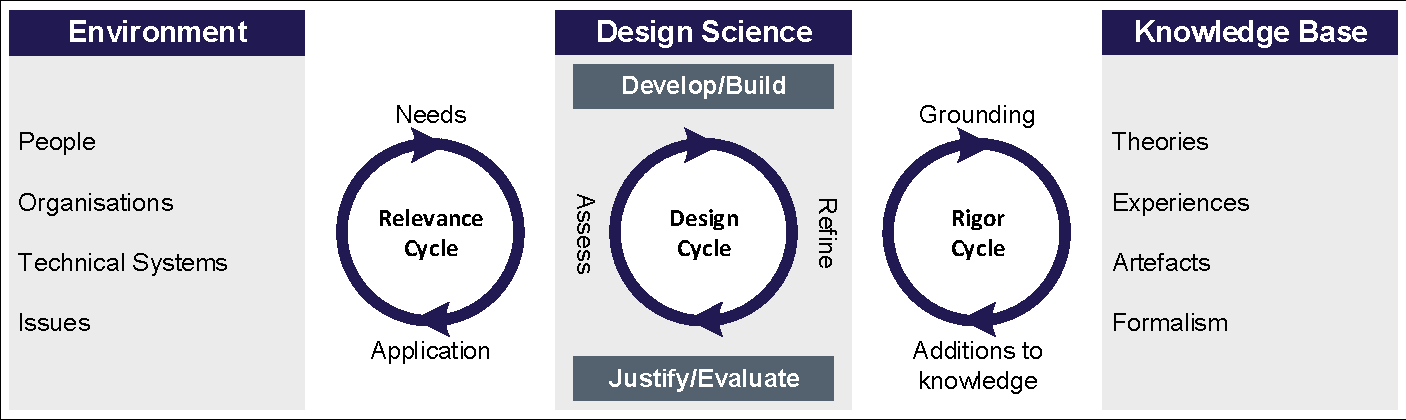
\includegraphics[width=\textwidth, trim=2 2 2 2, clip]{mainmatter/approach/figures/ISRframework.pdf}
  \caption{\posscite{Hevner2007TheTC} information systems framework and design science research cycles.}\label{fig:ISRframework}
\end{figure}
The \emph{relevance cycle} provides a context for application of the design science research results, along with a specification of the requirements and determination of acceptance criteria for evaluating the outcome of the research.
It connects the design activities to the overall context for the research project.
Needs are defined in the environment, \ie{} the problem space, and provide an input to be processed by design science activities.
Every artefact developed based on the needs from the environment is applied within the context of the environment, and field tested to determine the artefact's utility.
Through the \emph{rigor cycle}, the design activities are founded in scientific theories, experiences, and existing artefacts in a knowledge base while newly developed artefacts, theories, experiences, and potential extensions to already existing entries are fed back to the knowledge base.
Central to the design activities and project is the \emph{design cycle} itself.
In this cycle, the two core design activities of building (developing) and evaluating (justifying) are carried out iteratively.
Artefacts are built, evaluated, and refined until a satisfactory result is achieved.
The requirements upon which the evaluation is based are input from the relevance cycle, while the evaluation, development, and refinement methods are all pulled from the rigor cycle.
As \textcite{Hevner2007TheTC} put it, ``it is important to understand the dependencies of the design cycle on the other two cycles while appreciating its relative independence during the actual execution of research.''

The four types of artefacts are all highly relevant to the development of manufacturing system platforms.
Construct artefacts, defined as vocabulary and symbols, is essentially the language and manner in which problems and solutions are communicated and defined.
While the platforms are discussed increasingly frequently in research and within companies, there are still several individual understandings and opinions of \eg{} what constitutes a platform, how a module is defined, what a manufacturing process or manufacturing system is~\parencite{SorensenMCPC2017,SorensenAPMS2018}.
Developing constructs, \eg{} in the shape of employee handbooks, classification schemes, and modelling formalisms, makes communication during platform projects easier and helps avoid misunderstandings.
They also function as templates and forms for documenting platforms and their development.
Model \gls{glos:artefact}s use the vocabulary defined in constructs to represent the problem, solution, environment, and the link between them.
They are tools to be used during platform development, \eg{} to represent the functional structure of a platform in development, highlight how requirements are realised in the modules of a platform, or ways of representing entire manufacturing systems and their characteristics.
Abstracting various aspects of platforms in this manner is useful to manage the complexity of the development process.

Method \gls{glos:artefact}s are processes or procedures guiding problem solving and decision-making.
An informal method can be a simple text, describing how a manufacturing process is carried out, or how a model is built and used.
Method artefacts can also be formal mathematical algorithms, \eg{} providing a measure of the commonality between two systems, or a recommendation on which platforms to develop.
Instantiation \gls{glos:artefact}s are artefacts implemented to solve a problem in an environment.
This can, for instance, be the actual decision of selecting a potential platform based on an algorithm applied to a classification coding scheme.
An instantiation artefact may also be an implemented manufacturing system platform.
Examples of these are few and far between, but remain critical to the continued research within the field as a way to demonstrate the feasibility of both the platforms and the artefacts, theories, and experiences that helped create them.

The design science in information systems research framework outlined above is an appropriate fit for research on manufacturing system platforms since it is, as discussed in \cref{ssec:pPlatforms}, a field of relative immaturity.
Thus, the notion of employing knowledge bases aligns with, as others have suggested, gaining inspiration and applying concepts from other fields of research, thereby contributing to the knowledge base on manufacturing system platforms with new experiences and artefacts.
Further, with its focus on application of artefacts to solve real-world problems within a defined environment context, it lends itself well to case-studies, where new tools and methods are developed, or existing tools and methods are applied in a new context.
Another reason for choosing this framework, is that it is both proactive and reactive with respect to technology~\parencite{10.2307/25148625}.
Proactive, in the sense that design science focuses on creating and evaluating technology and artefacts, allowing the industry to address their needs through the artefacts.
Reactive, as behavioural science focuses on developing and justifying theories related to the implementation and use of technology and artefacts.
Research on platforms should be developed and evaluated in a collaborative context between academia and the industry.